% Table S1 - runtime and memory. Source of truth: ../benchmarks/SUPPLEMENTARY_TEXT.md
% Graphic: ../benchmarks/tableS1.pdf (vector, 186.9 x 38.4 mm -> 34.9 mm at 170 mm).
% NOTE: ../benchmarks/SUPPLEMENTARY_TEXT.md states this image is for circulating
% a draft and that the final version should be set in LaTeX. The data are in the
% markdown table in that file; converting it to a booktabs table like table1.tex
% would replace the \includegraphics line below.
% Requires: graphicx, array
% The graphic sits in a single-cell tabular because sn-jnl wraps table bodies in
% threeparttable, which silently drops the caption if the body has no tabular.
\begin{table}[t!]
\centering
\caption{\textbf{Runtime and memory for the three worked examples.} Each library
was generated at its published size on a single core. Times are means $\pm$ SD
over 5 replicate runs; peak memory is maximum resident set size, including a
$\sim$106~MB baseline for the Python interpreter, NumPy, and pandas. DAG
construction does not depend on library size and is reported separately.
The SpliceAI library comprises two matched 200,000-sequence pools (cryptic GT
and disrupted GA) generated separately; values are for one pool, and the full
library takes twice as long.}
\label{tab:runtime}
\begin{tabular}{@{}c@{}}
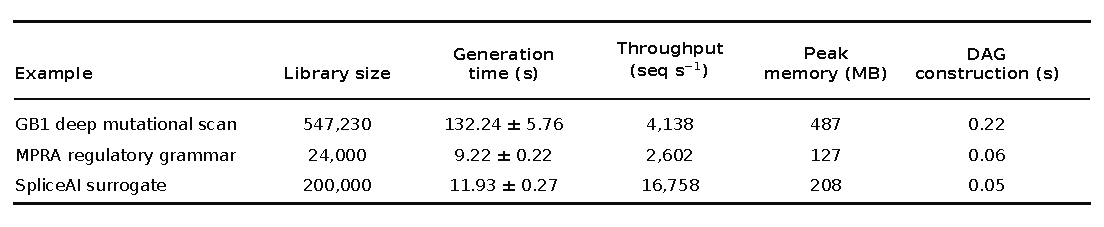
\includegraphics[width=\textwidth]{../benchmarks/tableS1}
\end{tabular}
\end{table}
